%%%%%%%%%%%%%%%%%%%%%%
% This is an example presentation made with Christopher Gandrud's unofficial LSE Beamer theme
% Updated 27 December 2011
%%%%%%%%%%%%%%%%%%%%%%

\documentclass[xcolor={svgnames,usenames}]{beamer}
\usetheme{LSE}
\usepackage{color}
\usepackage{hyperref}
\hypersetup{colorlinks=true,linkcolor=black}
\usepackage{graphics}
\usepackage{pgf,tikz,pgfplots}
\usetikzlibrary{shapes,arrows,intersections}
\usetikzlibrary{matrix,fit,calc,trees,positioning,arrows,chains,shapes.geometric,shapes}
\usetikzlibrary{decorations.pathmorphing,patterns}
\usepackage{booktabs}
\usepackage{minted}
\usepackage{nicefrac}

%%%%%%%%%%%%%%%%%%%%%%%%%%%%%%%% Title Slide %%%%%%%%%%%%%%%%%%%%%%%%%%
\title[Calcolo Parallelo]{Calcolo Parallelo : Lezione 1}
\author[F. Durastante]{
    \href{mailto:fabio.durastante@nunipi.it}{Fabio Durastante}
}
\institute{Dipartimento di Matematica, Università di Pisa}
\date[Maggio 2021]{Master in Scienze e Tecnologie Spaziali, 2022}

\beamerdefaultoverlayspecification{}

% ----------------
% Disegni Tikz per differenze finite
% ----------------
\pgfdeclarelayer{edgelayer}
\pgfdeclarelayer{nodelayer}
\pgfsetlayers{edgelayer,nodelayer,main}

\tikzstyle{none}=[inner sep=0pt]

\usetikzlibrary{decorations.markings}
\usetikzlibrary{shapes.geometric}

\tikzstyle{rn}=[circle,fill=Red,draw=Black,line width=0.8 pt,inner sep=0p]
\tikzstyle{gn}=[circle,fill=Lime,draw=Black,line width=0.8 pt]
\tikzstyle{yn}=[circle,fill=Yellow,draw=Black,line width=0.8 pt]

\tikzstyle{simple}=[-,draw=Black,line width=2.000]
\tikzstyle{arrow}=[-,draw=Black,postaction={decorate},decoration={markings,mark=at position .5 with {\arrow{>}}},line width=2.000]
\tikzstyle{tick}=[-,draw=Black,postaction={decorate},decoration={markings,mark=at position .5 with {\draw (0,-0.1) -- (0,0.1);}},line width=2.000]

\begin{document}

\begin{frame}
	\titlepage
\end{frame}

\section[Outline]{}
\frame[allowframebreaks]{\tableofcontents}

%%%%%%%%%%%%%%%%%%%%%%%%%%%%%%%%%
\section{Scientific and parallel computing}

\begin{frame}{Scientific and parallel computing}

\begin{columns}
	\begin{column}{0.6\textwidth}
		\begin{center}
		``\textbf{Computational science} (also \textbf{scientific computing} or \textbf{scientific computation} (SC)) is a rapidly growing multidisciplinary field that uses advanced computing capabilities to \emph{understand and solve complex problems}. It is an area of science which spans many disciplines, but at its core it involves the development of \emph{models and simulations to understand natural systems}.''
		\end{center}
		
		\flushright Wikipedia
	\end{column}
	\begin{column}{0.4\textwidth}
		\centering
		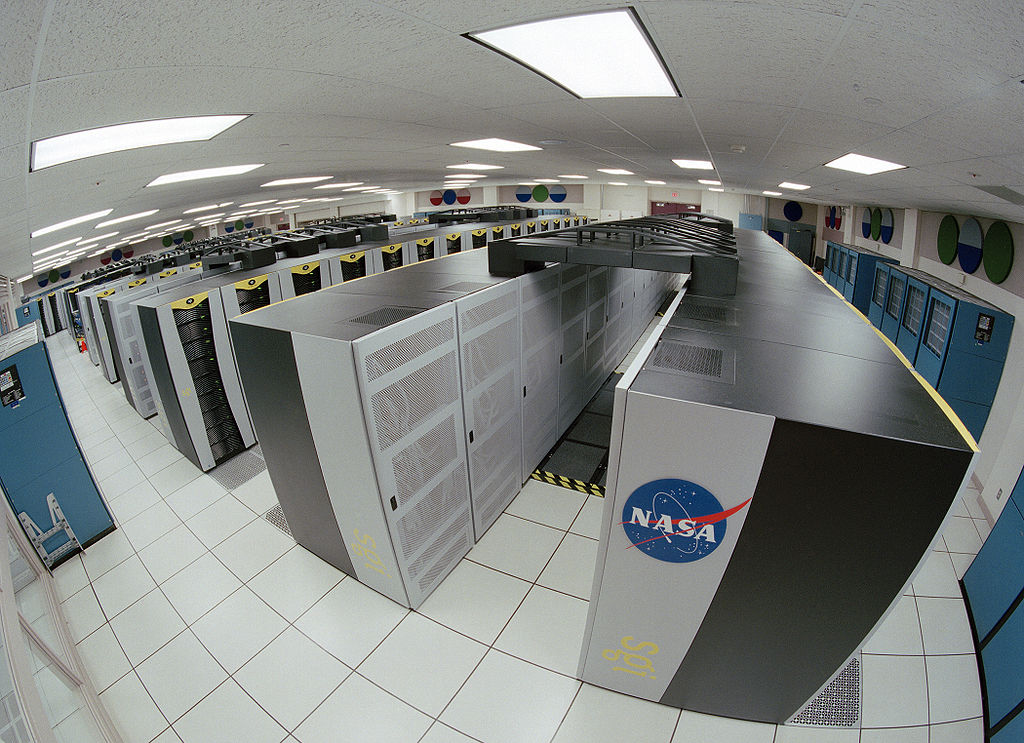
\includegraphics[width=\columnwidth]{nasasuperpc.jpg}
		
	\end{column}
\end{columns}

\end{frame}

\begin{frame}{What are the applications?}
	\centering
	\begin{columns}
		\begin{column}{0.5\textwidth}
		\begin{itemize}
		\item Computational finance,
		\item Computational biology,
		\item Simulation of complex systems,
		\item Network analysis
		\item Multi-physics simulations,
		\item Weather and climate models,
		\item \ldots 
		\end{itemize}
		\end{column}
		\begin{column}{0.5\textwidth}
			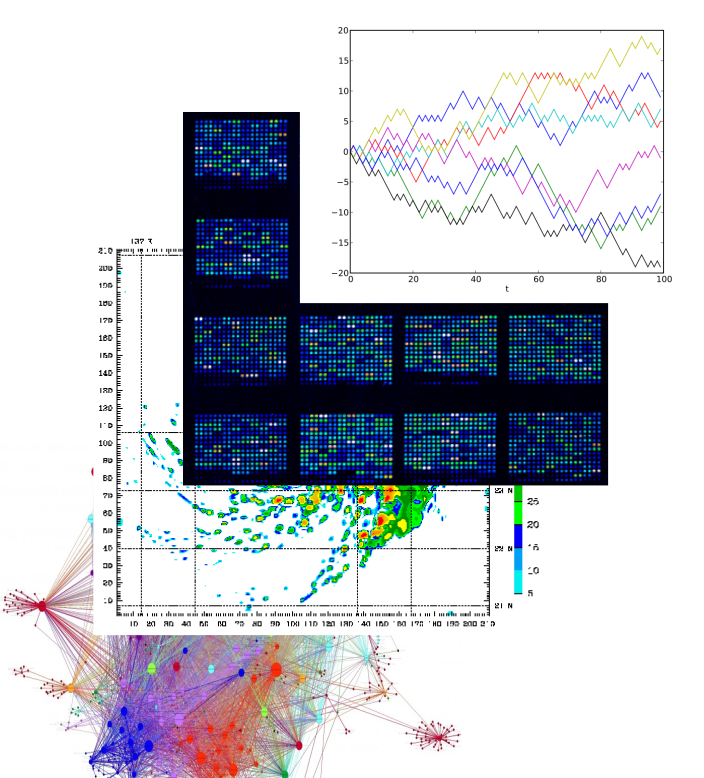
\includegraphics[width=\columnwidth]{applications.png}
		\end{column}
	\end{columns}
	\vfill
	\onslide<2>{Why the need for \alert{parallelism}?}
\end{frame}

\begin{frame}{Moore's law}
	\begin{columns}
		\begin{column}{0.4\columnwidth}
		\centering
		
\includegraphics[width=0.3\columnwidth]{Gordon_Moore.jpg}
		
		{\small
			``The complexity for minimum component costs has increased at a rate of roughly a factor of two per year. Certainly over the short term this rate can be expected to continue, if not to increase. Over the longer term, the rate of increase is a bit more uncertain, although there is no reason to believe it will not remain nearly constant for at least 10 years.''
		}
	
		{\flushright G. Moore, 1975}
		\end{column}
	\begin{column}{0.6\columnwidth}
		\centering
		
\includegraphics[width=\columnwidth]{mooreslawoftransistors.png}
		
		\onslide<2>{
		Computers \emph{should} reach the physical limits of Moore's Law at some point in the 2020s\ldots exponential functions saturates physical capabilities!
		}
	\end{column}
	\end{columns}
\end{frame}

\begin{frame}{Motivations for parallel computing}
\begin{itemize}
\item<1-> We are hitting the wall of single processor transistor count/computing capabilities,
\item<2-> Some applications needs more memory than the one that could be available on a single machine,
\item<3-> Optimization of sequential algorithms can bring us only to a certain extent
\end{itemize}
\onslide<4->{
	\centering
	``$\delta\iota\alpha\acute{\iota}\rho\epsilon\iota\,\kappa\alpha\grave{\iota}\,\beta\alpha\sigma\acute{\iota}\lambda\epsilon\nu\epsilon$``\\
	(di\'{a}irei k\'{a}i bas\'{i}leue)}

\onslide<5->{
\centering
Dividi et Impera
}

\onslide<6>{
\flushleft
Therefore, we need
\begin{itemize}
	\item Algorithms that can work in parallel,
	\item A communications protocol for parallel computation integrated with our programming languages
	\item Parallel machines that can actually run this code
\end{itemize}
}
\end{frame}

\subsection{Flynn's Taxonomy}

\begin{frame}{Parallel computers: Flynn's Taxonomy}
Let us start from the bottom: the \alert{machines}.
\begin{itemize}
	\item<2-> What is a parallel computer? \only<3-4>{well, it can be a certain number of different ``things''
	\begin{itemize}
		\item \alert<4>{Multi-core computing}
		\item Symmetric multiprocessing
		\item Distributed computing
		\item \alert<4>{Cluster computing}
		\item \alert<4>{Massively parallel computing}
		\item Grid computing
		\item \alert<4>{General-purpose computing on graphics processing units (GPGPU)}
		\item Vector processors
	\end{itemize}}
	\item<5-> Let us \emph{abstract} from the machine by describing Flynn's taxonomy 
	\begin{columns}
		\begin{column}{0.25\columnwidth}
		\centering
		\small
		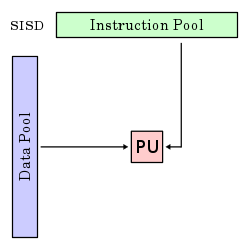
\includegraphics[width=\columnwidth]{SISD.png}
		
		Single instruction stream, single data stream\\SISD
		\end{column}
			\begin{column}{0.25\columnwidth}
						\centering
				\small
	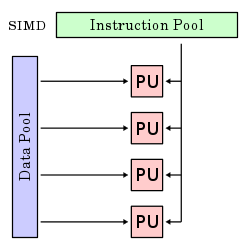
\includegraphics[width=\columnwidth]{SIMD.png}
	
	\alert<6>{Single instruction stream, multiple data streams\\SIMD}
	\end{column}
		\begin{column}{0.25\columnwidth}
					\centering
			\small
	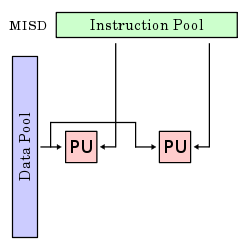
\includegraphics[width=\columnwidth]{MISD.png}
			
	Multiple instruction streams, single data stream\\MISD
\end{column}
\begin{column}{0.25\columnwidth}
					\centering
			\small
	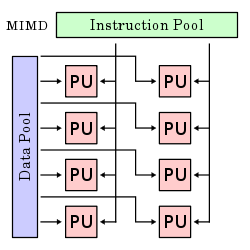
\includegraphics[width=\columnwidth]{MIMD.png}			
	
	\alert<6->{Multiple instruction streams, multiple data streams\\MIMD}
\end{column}
	\end{columns}
\end{itemize}
\end{frame}

\begin{frame}{Parallel Computers: our computer model}
For our task of introducing parallel computations we need to fix a \textbf{specific multiprocessor model}, i.e., a specific generalization of the sequential RAM model in which there is more than one processor.
\vfill
\begin{columns}
	\begin{column}{0.5\columnwidth}
	Since we want to stay in a SIMD/MIMD model, we focus on a \emph{local memory machine model}, i.e., a set of $M$ processors each with its own local memory that are attached to a common communication network.
	\end{column}
	\begin{column}{0.5\columnwidth}
	\centering
	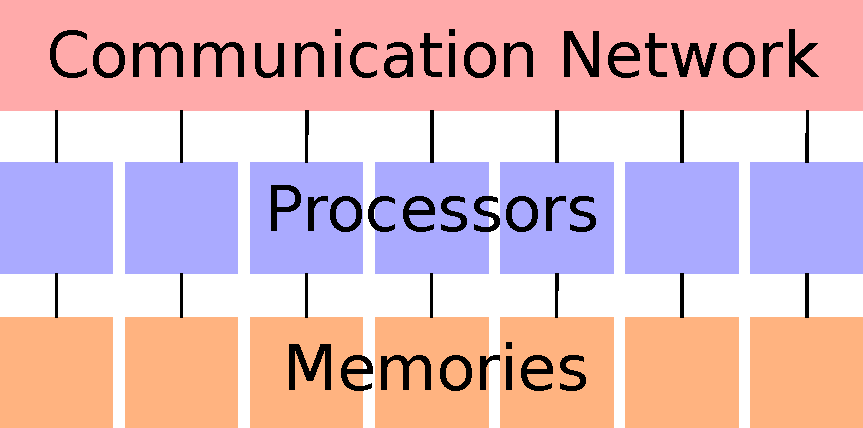
\includegraphics[width=\columnwidth]{networkarchitecture.pdf}
	\end{column}
\end{columns}
\vfill
\only<2>{
\begin{itemize}
	\item We can be more precise about the connection between processors, one can consider a network (a collection of switches connected by communication channels) and delve in a detailed way into its pattern of interconnection, i.e., into what is called the network topology.
\end{itemize}
}
\only<3>{
\begin{itemize}
	\item An alternative is to summarize the network properties in terms of two parameters: \alert{latency} and \alert{bandwidth}
	\begin{description}
		\item[Latency] the time it takes for a message to traverse the network;
		\item[Bandwidth] the rate at which a processor can inject data into the network.
	\end{description}
\end{itemize}
}


%\vfill
%\onslide<3>{
%	\centering
%	What are the available machines?
%}
\end{frame}


\subsection{The TOP500 List}

\begin{frame}{The TOP500 List -- \url{https://www.top500.org/}}
\begin{columns}
	\begin{column}{0.4\columnwidth}
	\small
	``\ldots we have decided in 1993 to assemble and maintain a list of the 500 most powerful computer systems. Our list has been compiled twice a year since June 1993 with the help of high-performance computer experts, computational scientists, manufacturers, and the Internet community in general\ldots
	
	In the present list (which we call the TOP500), we list computers ranked by their performance on the \alert{LINPACK Benchmark}.''
	\vfill
	\url{http://www.netlib.org/benchmark/hpl/}
	\end{column}
	\begin{column}{0.6\textwidth}
	\small
	\onslide<2>{
	The \alert{LINPACK} Benchmark.
	
	Solution of a dense $n\times n$  system of linear equations $A\mathbf{x} = \mathbf{b}$, so that
	\begin{itemize}
		\item $\frac{\| A \mathbf{x} - \mathbf{b}\|}{\|A\|\|\mathbf{x}\| n \varepsilon} \leq O(1)$, for $\varepsilon$ machine precision,
		\item It uses a specialized right--looking LU factorization with look--ahead
		\item Measuring 
		\begin{itemize}
			\item $R_\text{max}$ the performance in GFLOPS for the largest problem run on a machine,
			\item $N_\text{max}$ the size of the largest problem run on a machine,
			\item $N_{1/2}$ the size where half the $R_\text{max}$ execution rate is achieved,
			\item $R_{\text{peak}}$ the theoretical peak performance GFLOPS for the machine.
		\end{itemize}
	\end{itemize}
	
	

	}
	\end{column}
\end{columns}
\end{frame}
%
%
\section{Parallel Algorithms}

\begin{frame}{Parallel Algorithms}
In a fairly general way we can say that a \textbf{parallel algorithm} is an algorithm which can do \emph{multiple operations} in a given time.

\onslide<2->{\textbf{Example:} the sum of two vectors $\mathbf{x}, \mathbf{y} \in \mathbb{R}^n$

\begin{equation*}
	\begin{array}{cl}
	\mathbf{x} & = [x_1 \; x_2 \; \cdots \; x_i  \;\onslide<3>{\textcolor{blue}{\boldsymbol{|}}\;} x_{i+1} \; \cdots x_n] \\
	+ \\
	\mathbf{y} & = [y_1 \; y_2 \; \cdots \; y_i  \;\onslide<3>{\textcolor{blue}{\boldsymbol{|}}\;} y_{i+1} \; \cdots y_n] \\
	= \\
	\mathbf{x} + \mathbf{y} & = [x_1+y_1 \; x_2+y_2 \; \cdots \; x_i+y_i  \;\onslide<3>{\textcolor{blue}{\boldsymbol{|}}\;} \cdots x_n+y_n] \\
	\end{array}
\end{equation*}
\begin{itemize}
	\item<2-> If we do the operation sequentially we do $O(n)$ operations in $T_n$
	\item<3-> If we split the operation among $2$ processors, one summing up the entries between $1,\ldots,i$, and one summing up the entries between $i+1,\ldots,n$ we take $T_i$ time for the first part and $T_{n-i}$ time for the second, therefore the overall time is $\max(T_{i},T_{n-i})$ for doing always $O(n)$ operations.
\end{itemize}

}
\end{frame}

\begin{frame}{Parallel Algorithms: \emph{speedup}}\vspace{-0.8em}
\small
Let us try to think again in an abstract way and to quantify the \alert{overall speed gain} for a given gain in a subset of a process.
\begin{itemize}
	\item<1-> We break some process into $N$ distinct portions with the $i$th portion occupying the $P_i$ fraction of the overall completion time,
	\item<2-> then we order such portion in such a way that the $N$th portions subsumes all the parts of the overall processes that have fixed costs.
	\item<3-> The \emph{speedup} of the $i$th portion can then be defined as 
	\begin{equation*}
		S_i \triangleq \frac{t_{\text{original}}}{t_{\text{optimized}}}, \quad i=1,\ldots,N-1
	\end{equation*}
	where the numerator and denominator are the original and optimized completion time.
%	\item<4-> 
\end{itemize}
\begin{block}<4>{Amdahl's Law}
Then the \textcolor{blue}{overall speedup} for $\mathbf{P} = (P_1,\ldots,P_N)$, $\mathbf{S} = (S_1,\ldots,S_{N-1})$ is:
\begin{equation*}
S(\mathbf{P},\mathbf{S}) = \left(P_N + \sum_{i=1}^{N-1} \frac{P_i}{S_i}\right)^{-1}.
\end{equation*}
\end{block}

\end{frame}

\begin{frame}{Parallel Algorithms: \emph{Amdahl's Law}}
Let us make some observations on Amdahl's Law
\begin{itemize}
	\item We are not assuming about whether the original completion time  involves some optimization,
	\item We are not making any assumption on what our optimization process is,
	\item We are not even saying that the process in question involves a computer!
\end{itemize}
Amdahl's Law is a fairly general way of looking at how processes can be speed up by dividing them into sub-tasks with lower execution time. 

\onslide<2>{Moreover, it fixes  the \alert{theoretical maximum speedup} in various scenarios.
\begin{itemize}
	\item If we allow all components $S_i$ to grow unbounded then the upper bound on all scenario si $S_{\text{max}} = 1/P_N$.
\end{itemize}
Let us decline it in the context of the potential utility of \emph{parallel hardware}.
}
\end{frame}

\begin{frame}{Parallel Algorithms: \emph{Amdahl's Law} for \emph{parallel hardware}}
 Consider now having a parallel machine that permits us dividing the execution of code across $M$ hardware units, then the problem independent maximum speedup that such hardware can provide is $M$.
 \begin{block}{Parallel Efficiency}
 We define the parallel efficiency $E$ as
 \begin{equation*}
 	E \triangleq \frac{S_{\text{overall}}}{M},
 \end{equation*}
 where $E = 100\%$ correspond to the maximal use of the available hardware. When $S_{\text{max}} < M$, it is then impossible to take full advantage of all available execution units.
 \end{block}
\onslide<2->{\alert{Goal:} we require very large $S_{\text{max}}$ and correspondingly tiny $P_N$.}

\onslide<3->{\begin{center}
	\underline{Every dusty corner of a code must scale}, any portion that doesn't becomes the rate-limiting step!
\end{center}}
 
\end{frame}

\begin{frame}{Parallel Algorithms: \emph{Amdahl's Law} limitations}
What we are neglecting and what we are tacitly assuming
\begin{itemize}
	\item We are neglecting \emph{overhead costs}, i.e., the cost associated with parallel execution such as
	\begin{itemize}
		\item initializing (spawning) and joining of different computation threads,
		\item communication between processes, data movement and memory allocation.
	\end{itemize}
	\item We considered also the ideal case in which $S_i \rightarrow +\infty$ $\forall i$, observe that with finite speedup on portions $1$ through $N-1$, the $S_{\text{overall}}$ might continue to improve with increasing number of execution units.
	\item We are assuming that the size of the problem remains fixed while the number of execution units increases, this is called the case of \alert{strong scalability}. In some contexts, we need to turn instead to \alert{weak scalability} in which the problem size grows proportionally to the number of execution units.
\end{itemize}
\end{frame}

\section{Message Passing Interface}

\begin{frame}{How do we realize practically this parallelism?}
Let us focus on what we have discussed until now:
\begin{itemize}
	\item We have ``machines'' with multiple processors and whose main memory is partitioned into fragmented components,
	\item We have algorithms that can divide a problem of size $N$ among these processors so that they can run (almost) independently,
	\item With a certain degree of approximation, we know how to compute what is the \emph{best improvement} we can expect from a parallel program with $M$ processors on a problem of size $N$.
\end{itemize}
What we need to discuss now is then: ``How can we actually implement these algorithms on real machines?''
\begin{itemize}
	\item We need a way to define a parallel environment in which every processor is accounted for,
	\item We need to have data formats that are aware of the fact that we have a \emph{distributed} memory,
	\item We need to exchange data between the various memory fragments.
\end{itemize}
\end{frame}
%
\begin{frame}{Message Passing Interface -- \url{https://www.mpi-forum.org/}}

\begin{quote}
	``MPI (Message Passing Interface) is a \alert{specification for a standard library} for message passing that was defined by the MPI Forum, a broadly based group of parallel computer vendors, library writers, and applications specialists.'' -- W. Gropp, E. Lusk, N. Doss, A. Skjellum,
	\emph{A high-performance, portable implementation of the MPI message passing interface standard}, Parallel Computing, 22 (6), 1996.
\end{quote}

\begin{itemize}
	\item<2-> MPI implementations consist of a specific set of routines directly callable from C, C++, Fortran;
	\item<3-> MPI uses Language Independent Specifications for calls and language bindings;
	\item<4-> The MPI interface provides an essential \emph{virtual} topology, synchronization, and communication functionality inside a set of processes.
	\item<5-> There exist many implementations of the MPI specification, e.g., MPICH, Open MPI, pyMPI
\end{itemize}
\end{frame}

\subsection{Our First MPI Program}

\begin{frame}[fragile]{Hello (parallel) world!}
In all the course we are going to use the MPI inside C programs.
\begin{columns}
\begin{column}{0.4\columnwidth}
\begin{minted}{c}
#include"mpi.h"
#include<stdio.h>

int main(int argc, 
	char **argv){
 MPI_Init( &argc, &argv);
 printf("Hello, world!\n");
 MPI_Finalize();
 return 0;
}
\end{minted}
\end{column}
\begin{column}{0.56\columnwidth}
\small
\begin{itemize}
	\item \mintinline{c}{#include "mpi.h"} provides basic MPI definitions and types,
	\item \mintinline{c}{MPI_Init} start MPI, it has to precede any MPI call!
	\item \mintinline{c}{MPI_Finalize} exits MPI
	\item All the non--MPI routines are local!
\end{itemize}
\end{column}
\end{columns}
\vfill
\onslide<2>{We need now to \emph{compile} and \emph{link} the \mintinline{console}{helloworld.c} program, and we can do it simply by:
\
\mint{bash}{mpicc helloworld.c -o helloworld}
}
\end{frame}

\begin{frame}[fragile]{Hello (parallel) world! -- Compile, Link and Run}
\mint{bash}{mpicc helloworld.c -o helloworld}
\begin{itemize}
	\item \mintinline{console}{mpicc} is a wrapper for a C compiler provided by the Open MPI implementation of MPI.
	\item the option \mintinline{console}{-o} sets the name of the compiled (executable) file.
\end{itemize}
\onslide<2->{Let us see what is happening behind the curtains}
\begin{itemize}
\item<2-> you can first try to discover what compiler are you using by executing \mintinline{console}{mpicc --version}, \begin{onlyenv}<2>
that will give you something like
\begin{minted}{console}
icc (ICC) 17.0.4 20170411
Copyright (C) 1985-2017 Intel Corporation.  
All rights reserved.
\end{minted} 
for an Intel compiler.
\end{onlyenv}
\item<3-> or discover what are the library inclusion and linking options by asking for \mintinline{console}{mpicc --showme:compile} and \mintinline{console}{mpicc --showme:link}, respectively.
\item<4-> In general, looking at the output of the \mintinline{console}{man mpicc} command is always a good idea.
\end{itemize} 
\only<5>{{\centering\small``If you find yourself saying, "But I don't want to use wrapper compilers!", please humor us and try them. See if they work for you. Be sure to let us know if they do not work for you. '' - {\scriptsize \url{https://www.open-mpi.org/faq/?category=mpi-apps}}}}
\end{frame}

\begin{frame}[fragile]{Hello (parallel) world! -- Compile, Link and Run}
A piece of advice: if your program is anything more realistic than a classroom exercise use \mintinline{console}{make}\footnote{\url{https://www.gnu.org/software/make/}}, and save yourself from writing painfully long compiling commands, and dealing with complex dependencies more than once.

\begin{quote}
``Make gets its knowledge of how to build your program from a file called the makefile, which lists each of the non-source files and how to compute it from other files.''
\end{quote}

A very simple \mintinline{console}{Makefile} for our first test would be
\begin{minted}{Makefile}
MPICC = mpicc #The wrapper for the compiler
CFLAGS += -g  #Useful for debug symbols
all: helloworld
helloworld: helloworld.c
  $(MPICC) $(CFLAGS) $(LDFLAGS) $? $(LDLIBS) -o $@
clean:
  rm -f helloworld
\end{minted}
\end{frame}

\begin{frame}[fragile]{Hello (parallel) world! -- Compile, Link and Run}
If you are running on your machine (possibly for doing some debug), you can run your first parallel program by doing:
\mint{bash}{mpirun [ -np X ] [ --hostfile <filename> ]  helloworld}
or by using its synonym
\mint{bash}{mpiexec [ -np X ] [ --hostfile <filename> ]  helloworld}
\begin{itemize}
	\item<1-> \mintinline{console}{mpirun}/\mintinline{console}{mpiexec} will  run  \mintinline{console}{X} copies of \mintinline{console}{helloworld} in your current run-time environment, scheduling (by default) in a round-robin fashion by CPU slot.
	\item<1-> if running under a supported resource manager, Open MPI's \mintinline{console}{mpirun} will usually automatically use the corresponding resource manager process starter, as opposed to, for example, rsh or ssh, which require the use of a hostfile, or will default  to  running all \mintinline{console}{X} copies on the localhost 
	\item<2-> as always, look at the manual, by doing \mintinline{console}{man mpirun}.
\end{itemize}

\end{frame}

\begin{frame}{Queue management systems}
To run on a shared machine you will most certainly encounter a \emph{so-called} queue management system/workload manager, usually one between
\begin{itemize}
	\item SLURM \href{https://slurm.schedmd.com/}{slurm.schedmd.com}
	\item PBS \href{https://www.openpbs.org/}{www.openpbs.org}
\end{itemize}
They are ``fault-tolerant, and highly scalable cluster management and job scheduling system for large and small Linux clusters.'', meaning:
\begin{itemize}
	\item You don't simply run \mintinline{console}{mpirun}/\mintinline{console}{mpiexec} asking for resources on a shared machine, with many users chaos would immediately follow,
	\item You \textbf{ask for resources} for your \textbf{job} and put it into an \textbf{execution queue}. 
	\item When the resources you need will be available your program will be executed (for the requested amount of time)
\end{itemize}

On the machine we use for this course we have \alert{SLURM} installed, so we are going to give usage details only about it.

\end{frame}

\begin{frame}[fragile]{SLURM: basic usage}\vspace{-1em}
The \alert{key idea} is that we produce a bash script containing the information on what we want to be executed and give it to SLURM to put into the queue.

We create a file \verb|run-helloworld.sh| with
\begin{minted}[fontsize=\scriptsize]{bash}
#!/bin/bash
#SBATCH --job-name=helloworld      # Job name (can be called with %x)
#SBATCH --partition=Prod           # Node partition: here only Prod
#SBATCH --nodes=1                  # Run all processes on a single node
#SBATCH --ntasks=6                 # Run ntasks processes (-np ntasks)
#SBATCH --time=00:05:00            # Time limit hrs:min:sec
#SBATCH -o ./%x.%j.out             # Standard Output (%j job number)
#SBATCH -e ./%x.%j.err             # Standard Error  (%j job number)
mpirun helloworld
\end{minted}

Then we put it into the queue by doing \mint{bash}{sbatch run-helloworld.sh}

To see if the \textbf{job} has been put into the queue (or executed) you can use the command \mintinline{bash}{squeue}, if you are on a machine that has many user and a long queue you may need to trim down the list by doing, e.g., \mintinline{bash}{squeue | grep parallel_job} that will search in the list just the job with your name.

\end{frame}

\begin{frame}{SLURM: basic usage}
There are (a lot) more options that can be used in SLURM, not all of them make sense for all programming models.

Other commands that are useful are:
\begin{description}
	\item[{\mintinline{bash}{sinfo}}] reports the state of partitions and nodes managed by Slurm. It has a wide variety of filtering, sorting, and formatting options.
	\item[{\mintinline{bash}{scancel}}] is used to cancel a pending or running job or job step. It can also be used to send an arbitrary signal to all processes associated with a running job or job step.
\end{description}

\textbf{Important.} If you request a combination of resources that does not make sense for SLURM, e.g., more nodes than you have, wrong partition, more time than possible, a non-matching set of nodes and tasks, then \alert{the job will fail on execution}. This means that you may end up waiting lot of time to be executed, and then fail with no answer whatsoever. Some unreasonable combination (e.g., unknown partition) may by noticed by \mintinline{bash}{sbatch}, but don't count on it.

\end{frame}


\begin{frame}[fragile]{Hello (parallel) world! -- Compile, Link and Run}
If we now run 
\mint{bash}{sbatch run-helloworld.sh}
we get a \mintinline{bash}{helloworld.xx.out} file containing the following output:
\begin{columns}
\begin{column}{0.4\columnwidth}
\begin{minted}{console}
Hello, world!
Hello, world!
Hello, world!
Hello, world!
Hello, world!
Hello, world!
\end{minted}
\end{column}
\begin{column}{0.6\columnwidth}
Every process executes the line \mint{c}{printf("Hello, world!\n");} that it is a \alert{local} routine!
\end{column}
\end{columns}
\begin{block}<2>{local vs non-local procedure}
	A procedure is \textbf{local} if completion of the procedure depends only on the local executing process.
	
	A procedure is \textbf{non-local} if completion of the operation may require the execution of some MPI procedure on another process. Such an operation \emph{may require
	communication} occurring with another user process.
\end{block}
\end{frame}

\subsection{The MPI parallel environment}
\begin{frame}[fragile]{The MPI parallel environment}
Let us modify our \mintinline{console}{helloworld} to investigate the MPI parallel environment. Specifically, we want to answer, from within the program, to the questions:
\begin{enumerate} 
	\item How many processes are there?
	\item Who am I?
\end{enumerate}
\begin{minted}{c}
#include "mpi.h"
#include <stdio.h>
int main( int argc, char **argv ){
 int rank, size;
 MPI_Init( &argc, &argv );
 MPI_Comm_rank( MPI_COMM_WORLD, &rank );
 MPI_Comm_size( MPI_COMM_WORLD, &size );
 printf( "Hello world! I'm process %d of %d\n",rank, size );
 MPI_Finalize();
 return 0;
}
\end{minted}
\end{frame}

\begin{frame}[fragile]{The MPI parallel environment}
\begin{minted}{c}
#include "mpi.h"
#include <stdio.h>
int main( int argc, char **argv ){
 int rank, size;
 MPI_Init( &argc, &argv );
 MPI_Comm_rank( MPI_COMM_WORLD, &rank );
 MPI_Comm_size( MPI_COMM_WORLD, &size );
 printf( "Hello world! I'm process %d of %d\n",rank, size );
 MPI_Finalize();
 return 0;
}
\end{minted}
\begin{itemize}
	\item How many is answered by a call to \mintinline{c}{MPI_Comm_size} as an \mintinline{c}{int} value,
	\item Who am I? Is answered by a call to \mintinline{c}{MPI_Comm_rank} as an \mintinline{c}{int} value that is conventionally called \mintinline{c}{rank} and is a number between \mintinline{c}{0} and \mintinline{c}{size-1}.
\end{itemize}
\end{frame}


\begin{frame}{The MPI parallel environment}
	The last keyword we need to describe is the \mintinline{c}{MPI_COMM_WORLD}, this is the standard Communicator object.

	\begin{block}{Communicator}
	A Communicator object connects a group of processes in one MPI session. There can be more than one communicator in an MPI session, each of them gives each contained process an independent identifier and arranges its contained processes in an ordered topology.
	\end{block}

	This provides
	\begin{itemize}
	\item a safe communication space, that guarantees that the code can communicate as they
	need to, without conflicting with communication extraneous to the present code, e.g., if other parallel libraries are in use,
	\item a unified object for conveniently denoting communication context, the group of communicating processes and to house abstract process naming.
	\end{itemize}
\end{frame}

\begin{frame}[fragile]{The MPI parallel environment}
If we have saved our inquiring MPI program in the file \mintinline{console}{hamlet.c}, we can then modify our \mintinline{console}{Makefile} by modifying/adding the lines
\begin{minted}{Makefile}
all: helloworld hamlet
hamlet: hamlet.c
 $(MPICC) $(CFLAGS) $(LDFLAGS) $? $(LDLIBS) -o $@
clean:
 rm -f helloworld hamlet
\end{minted}
Then, we compile everything by doing \mintinline{console}{make hamlet} (or, simply, \mintinline{console}{make}).

\begin{onlyenv}<2->
When we run the code with \mintinline{console}{mpirun -np 6 hamlet} we see
\begin{columns}
\begin{column}{0.5\columnwidth}
\begin{verbatim}
Hello world! I'm process 1 of 6
Hello world! I'm process 5 of 6
Hello world! I'm process 0 of 6
Hello world! I'm process 3 of 6
Hello world! I'm process 2 of 6
Hello world! I'm process 4 of 6
\end{verbatim}
\end{column}
\begin{column}{0.5\columnwidth}
\begin{itemize}
	\item<3-> Every processor answers the call,
	\item<4-> But it answers it as soon as he has done doing the computation! There is \alert{no synchronization}.
\end{itemize}
\end{column}
\end{columns}
\end{onlyenv}
\end{frame}

\subsection{When to travek the MPI road}
\begin{frame}{A word of advice}
When should you \textbf{not} write parallel code with MPI?
\begin{itemize}
	\item<1-> The effort of writing optimized and scalable MPI codes is not negligible, therefore a direct usage of it its usually best suited for developing \emph{libraries for scientific computations}. 
	\item<2-> If there is a library containing a good (possibly open source) parallel implementation of the algorithm and the data structure you need: LEARN IT AND USE IT!
\end{itemize}
When should you write parallel code with MPI?
\begin{itemize}
	\item<3-> When you are learning about parallel computing with distributed memory!
	\item<4-> To \emph{really} understand what the instructions manuals of such parallel libraries are telling you,
	\item<5-> Sometimes it happens, you are using a library based on MPI and some function that you truly need is not included. 
	\item<6-> To develop new and better libraries for your scientific challenge!
\end{itemize}
\end{frame}

\section{Point-to-Point Communications}

\begin{frame}[fragile]{Sending and Receiving Messages}
We have seen that each process within a \emph{communicator} is identified by its \emph{rank}, how can we \alert{exchange data} between two processes?
\begin{center}
	\begin{tikzpicture}
	\node[draw] (P0) at (0,0) {$P_0$};
	\node[draw] (P1) at (4,0) {$P_1$};
	\draw[-,dashed] (2,1) to (2,-2);
	\node[circle,draw=black,fill=white](A) at (0,-1) {$A$};
	\node[circle,draw=black,fill=white](B) at (4,-1.5) {$B$};
	\draw[->,thick] (A) -- +(2,0) |-  node[pos=.25] {} (B);
	\node at (1.2,-0.8) {\mintinline{c}{send}};
	\node at (2.8,-1.3) {\mintinline{c}{receive}};
	\end{tikzpicture}
\end{center}
We need to posses several information to have a meaningful message
\begin{itemize}
	\item Who is sending the data?
	\item To whom the data is sent?
	\item What type of data are we sending?
	\item How does the receiver can identify it?
\end{itemize}
\end{frame}

\begin{frame}[fragile]{The blocking send and receive}
\begin{minted}{c}
int MPI_Send(void *message, int count, 
MPI_Datatype datatype, int dest, int tag, 
MPI_Comm comm)
\end{minted}
\begin{description}
\item[\textcolor{black}{\mintinline{c}{void *message}}] points to the message content itself, it can be a simple scalar or a group of data,
\item[\textcolor{black}{\mintinline{c}{int count}}] specifies the number of data elements of which the message is composed,
\item[\textcolor{black}{\mintinline{c}{MPI_Datatype datatype}}] indicates the \alert{data type} of the elements that make up the message,
\item[\textcolor{black}{\mintinline{c}{int dest}}] the rank of the destination process, 
\item[\textcolor{black}{\mintinline{c}{int tag}}] the user-defined tag field, 
\item[\textcolor{black}{\mintinline{c}{MPI_Comm comm}}] the communicator in which the source and destination processes reside and for which their respective
ranks are defined.
\end{description}
\end{frame}

\begin{frame}[fragile]{The blocking send and receive}
\begin{minted}{c}
int MPI_Recv (void *message, int count, 
MPI_Datatype datatype, int source, int tag,
MPI_Comm comm, MPI_Status *status)
\end{minted}
\begin{description}
\item[\textcolor{black}{\mintinline{c}{void *message}}] points to the message content itself, it can be a simple scalar or a group of data,
\item[\textcolor{black}{\mintinline{c}{int count}}] specifies the number of data elements of which the message is composed,
\item[\textcolor{black}{\mintinline{c}{MPI_Datatype datatype}}] indicates the \alert{data type} of the elements that make up the message,
\item[\textcolor{black}{\mintinline{c}{int source}}] the rank of the source process, 
\item[\textcolor{black}{\mintinline{c}{int tag}}] the user-defined tag field, 
\item[\textcolor{black}{\mintinline{c}{MPI_Comm comm}}] the communicator in which the source and destination processes reside,
\item[\textcolor{black}{\mintinline{c}{MPI_Status *status}}] is a structure that contains three fields named \mintinline{c}{MPI_SOURCE} , \mintinline{c}{MPI_TAG}, and \mintinline{c}{MPI_ERROR}.
\end{description}
\end{frame}

\begin{frame}{Why ``blocking'' send and receive?}
For the \mintinline{c}{MPI_Send} to be \alert{blocking} means that it does not return until the message
data and envelope have been safely stored away so that the sender is free to modify the
send buffer: it is a \emph{non local} operation. 
\vfill
\begin{onlyenv}<1>
\alert{Note:} The message might be copied directly into the matching receive buffer (as in the first figure), or it
might be copied into a temporary system buffer.
\begin{center}
\begin{tikzpicture}
\node[draw] (P0) at (0,0) {$P_0$};
\node[draw] (P1) at (4,0) {$P_1$};
\draw[-,dashed] (2,1) to (2,-2);
\node[circle,draw=black,fill=white](A) at (0,-1) {$A$};
\node[draw=black,fill=green](B) at (4.3,-1.5) {Buffer};
\node[circle,draw=black,fill=white](C) at (6,-1.5) {$B$};
\draw[->,thick] (A) -- +(2,0) |-  node[pos=.25] {} (B);
\draw[->,thick] (B) to (C);
\node at (1.2,-0.8) {\mintinline{c}{send}};
\node at (2.8,-1.3) {\mintinline{c}{receive}};
\end{tikzpicture}
\end{center}
\end{onlyenv}
\only<2>{\vfill
The \mintinline{c}{MPI_Receive}, on the other hand returns \alert{only} after the receive buffer contains the newly received message. A receive can't complete before the matching send has completed, but, of course, it can complete only after the matching send has started.}
\end{frame}

\begin{frame}[fragile]{A simple send/receive example}
\footnotesize
\begin{minted}{c}
#include "mpi.h"
#include <string.h>
#include <stdio.h>
int main( int argc, char **argv){
char message[20];
int myrank;
MPI_Status status;
MPI_Init( &argc, &argv );
MPI_Comm_rank( MPI_COMM_WORLD, &myrank );
if (myrank == 0){  /* code for process zero */
strcpy(message,"Hello, there");
MPI_Send(message, strlen(message)+1, MPI_CHAR, 1, 99, MPI_COMM_WORLD);
}
else if (myrank == 1){ /* code for process one */
MPI_Recv(message, 20, MPI_CHAR, 0, 99, MPI_COMM_WORLD, &status);
printf("received :%s:\n", message);
}
MPI_Finalize();
return 0;
}
\end{minted}
\end{frame}

\begin{frame}[fragile]{A simple send/receive example}
\small
We can compile our code by simply adding to our \mintinline{bash}{Makefile} 
\begin{minted}{Makefile}
easysendrecv: easysendrecv.c
$(MPICC) $(CFLAGS) $(LDFLAGS) $? $(LDLIBS) -o $@
\end{minted}
then, we type \mintinline{bash}{make}, and we run our program with \mint{bash}{mpirun -np 2 easysendrecv} getting as answer
\begin{verbatim}
received :Hello, there:
\end{verbatim}
So, what have we done?
{\scriptsize \mint{c}{MPI_Send(message, strlen(message)+1, MPI_CHAR, 1, 99, MPI_COMM_WORLD);}}
Process $0$ sends the content of the \mintinline{c}{char} array \mintinline{c}{message[20]}, whose size is \mintinline{c}{strlen(message)+1} size of \mintinline{c}{char} (\mintinline{c}{MPI_CHAR}) to processor \mintinline{c}{1} with tag \mintinline{c}{99} on the communicator \mintinline{c}{MPI_COMM_WORLD}.
{\scriptsize \mint{c}{MPI_Recv(message, 20, MPI_CHAR, 0, 99, MPI_COMM_WORLD, &status);}}
on the other side process $1$, receives into the buffer \mintinline{c}{message[20]} an array with size \mintinline{c}{20} size of \mintinline{c}{MPI_CHAR}, from process \mintinline{c}{0} with tag \mintinline{c}{99} on the same communicator \mintinline{c}{MPI_COMM_WORLD}.
\end{frame}

\begin{frame}{A simple send/receive example : programmer smash!}
It is a good exercise to try and mess things up, so let us see some damaging suggestions:
\begin{itemize}
\item<1-> What happens if we have a mismatch in the tags?
\item[A:]<2-> The process stays there hanging waiting for a message with a tag that will never come\ldots 
\item<1-> What happens if we have a mismatch in the ranks of the sending and receiving processes?
\item[A:]<3-> The process stays there hanging trying to match messages that will never come\ldots 
\item<1-> What happens if we use the wrong message size?
\item[A:]<4-> If the size of the arriving message is longer than the expected we get an error of \mintinline{bash}{MPI_ERR_TRUNCATE: message truncated}, note that there are combinations of wrong sizes for which things still works
\item<1-> What happens if we have a mismatch in the type?
\item[A:]<5-> There are combinations of instances in which things seems to work, \alert{but} the code is erroneous, and the behavior is not deterministic.
\end{itemize}
\end{frame}

\subsection{Deadlock}

\begin{frame}[fragile]{Dealing with more than one send and receive}
We have now two processes that needs to exchange some data

\begin{onlyenv}<1-2>
\begin{itemize}
\item Solution 1:
\end{itemize}
{\footnotesize
\begin{minted}{c}
MPI_Comm_rank(comm, &myrank);
if (myrank == 0){
MPI_Send(sendbuf, count, MPI_DOUBLE, 1, tag, comm);
MPI_Recv(recvbuf, count, MPI_DOUBLE, 1, tag, comm, status);
}else if(myrank == 1){
MPI_Send(sendbuf, count, MPI_DOUBLE, 0, tag, comm); 
MPI_Recv(recvbuf, count, MPI_DOUBLE, 0, tag, comm, status);
}
\end{minted}
}
\end{onlyenv}

\begin{onlyenv}<2-3>
\begin{itemize}
\item Solution 2:
\end{itemize}
{\footnotesize
\begin{minted}{c}
MPI_Comm_rank(comm, &myrank);
if (myrank == 0){
MPI_Recv(recvbuf, count, MPI_DOUBLE, 1, tag, comm, status);
MPI_Send(sendbuf, count, MPI_DOUBLE, 1, tag, comm);
}else if(myrank == 1){ 
MPI_Recv(recvbuf, count, MPI_DOUBLE, 0, tag, comm, status);
MPI_Send(sendbuf, count, MPI_DOUBLE, 0, tag, comm);
}
\end{minted}
}
\end{onlyenv}

\begin{onlyenv}<3>
\begin{itemize}
\item Solution 3:
\end{itemize}
{\footnotesize
\begin{minted}{c}
MPI_Comm_rank(comm, &myrank);
if (myrank == 0){
MPI_Send(sendbuf, count, MPI_DOUBLE, 1, tag, comm);
MPI_Recv(recvbuf, count, MPI_DOUBLE, 1, tag, comm, status);
}else if(myrank == 1){
MPI_Recv(recvbuf, count, MPI_DOUBLE, 0, tag, comm, status);
MPI_Send(sendbuf, count, MPI_DOUBLE, 0, tag, comm); 
}
\end{minted}
}
\end{onlyenv}
\vfill
\end{frame}

\begin{frame}[fragile]{Dealing with more than one send and receive}
\small
\begin{columns}
\begin{column}{0.30\columnwidth}
\only<2,4>{
\centering

\includegraphics[width=\columnwidth]{Deadlock.pdf}

Here what happens to your program when you encounter Deadlock
}
\only<6>{
\centering

\includegraphics[width=\columnwidth]{Nodeadlock.jpg}

This way you can beat Deadlock!
}
\end{column}
\begin{column}{0.70\columnwidth}
\begin{onlyenv}<1-2>
\noindent In the case of Solution 1:
{\footnotesize
\begin{minted}{c}
MPI_Comm_rank(comm, &myrank);
if (myrank == 0){
 MPI_Send(...);
 MPI_Recv(...);
}else if(myrank == 1){
 MPI_Send(...); 
 MPI_Recv(...);
}
\end{minted}
}
\begin{itemize}
	\item The call \mintinline{c}{MPI_Send} is blocking, therefore the message sent by each process has to be copied out before the send operation returns
	and the receive operation starts.
	\item For the call to complete successfully, it is then necessary that \alert{at least one of the two messages sent be buffered}, otherwise \ldots
	\item a deadlock situation occurs: both processes are blocked since there is no buffer space available!
\end{itemize}
\end{onlyenv}
\begin{onlyenv}<3-4>
\noindent In the case of Solution 2:
{\footnotesize
\begin{minted}{c}
MPI_Comm_rank(comm, &myrank);
if (myrank == 0){
 MPI_Recv(...);
 MPI_Send(...);
}else if(myrank == 1){
 MPI_Recv(...);
 MPI_Send(...); 
}
\end{minted}
}
\begin{itemize}
	\item The receive operation of process $0$ must complete before its send. It can complete
	\alert{only if} the matching send of processor $1$ is executed.
	\item The receive operation of process $1$ must complete before its send. It can complete
	\alert{only if} the matching send of processor $0$ is executed.
	\item This program will always deadlock.
\end{itemize}
\end{onlyenv}
\begin{onlyenv}<5-6>
\noindent In the case of Solution 3:
{\footnotesize
\begin{minted}{c}
MPI_Comm_rank(comm, &myrank);
if (myrank == 0){
 MPI_Send(...);
 MPI_Recv(...);
}else if(myrank == 1){
 MPI_Recv(...);
 MPI_Send(...); 
}
\end{minted}
}
\begin{itemize}
	\item This program will succeed even if no buffer space for data is available.
\end{itemize}
\end{onlyenv}
\end{column}
\end{columns}	
\end{frame}

\begin{frame}[fragile]{Deadlock Issues}

We can try to salvage what the situation in the case of Solution 1 by allocating the buffer space for the send calls
\vfill
\begin{columns}
\begin{column}{0.3\columnwidth}
{\footnotesize
\begin{minted}{c}
if (myrank == 0){
 MPI_Send(...);
 MPI_Recv(...);
}else if(myrank == 1){
 MPI_Send(...); 
 MPI_Recv(...);
}
\end{minted}
}
\end{column}
\begin{column}{0.7\columnwidth}
\noindent We can substitute the \mintinline{c}{MPI_Send} operation with a Send in buffered mode
{\footnotesize
\begin{minted}{c}
int MPI_Bsend(const void* buf, int count, 
MPI_Datatype datatype, int dest,
int tag, MPI_Comm comm)
\end{minted}
}
\begin{itemize}
\item A buffered mode send operation can be started whether or not a matching receive
has been posted;
\item It may complete before a matching receive is posted;
\item This operation is \emph{local}!
\only<2>{\item The bad news is that if the buffer space is not enough we have exchanged the deadlock error with a \alert{buffer overflow condition};}
\only<3>{\item The good news is that buffer overflow condition are easier to detect than deadlock.}
\end{itemize}
\end{column}
\end{columns}

\end{frame}

\begin{frame}[fragile]{Allocating buffer space}
To actually use the \mintinline{c}{MPI_Bsend} we need also to allocate the space for the buffer, therefore we need to use the two functions
\mint{c}{int MPI_Buffer_attach(void* buffer, int size)}
\mint{c}{int MPI_Buffer_detach(void* buffer_addr, int* size)}
\only<1>{
\begin{itemize}
\item \mintinline{c}{MPI_Buffer_attach} provides a buffer in the user's memory to be used for buffering outgoing messages, where \mintinline{c}{buffer} is the starting address of a memory region
\item \mintinline{c}{MPI_Buffer_detach} detaches the buffer currently associated with MPI. The call returns the address and the
size of the detached buffer. \alert{This operation will block until all messages currently in the
buffer have been transmitted}.
\end{itemize}}
\begin{onlyenv}<2>
\begin{minted}{c}
#define BUFFSIZE 10000
int size; char *buff;
// Buffer of 10000 bytes for MPI_Bsend
MPI_Buffer_attach( malloc(BUFFSIZE), BUFFSIZE);
// Buffer size reduced to zero 
MPI_Buffer_detach( &buff, &size);
// Buffer of 10000 bytes available again 
MPI_Buffer_attach( buff, size); 
\end{minted}
\alert{Note:} a pointer to the buffer is passed to \mintinline{c}{MPI_Buffer_attach} while the address of the
pointer is passed to \mintinline{c}{MPI_Buffer_detach} and these are both \mintinline{c}{void *}.
\end{onlyenv}
\end{frame}

\subsection{Nonblocking communications}
\begin{frame}{Nonblocking communications}
As we have seen the use of blocking communications ensures that
\begin{itemize} 
\item the send and receive buffers used in the \mintinline{c}{MPI_Send} and \mintinline{c}{MPI_Recv}
arguments are safe to use or reuse after the function call, 
\item but it also means that unless there is a simultaneously matching send for each receive, the code will deadlock.
\end{itemize}

There exists a version of the point-to-point communication that \alert{returns immediately} from the function call before
confirming that the send or the receive has completed, these are the nonblocking send and receive functions.
\begin{itemize}
\item<2-> To verify that the data has been copied out of the send
buffer a separate call is needed,
\item<2-> To verify that the data has been received into the receive buffer a separate call is needed,
\item<3-> The sender should not modify any part of the send buffer after a nonblocking
send operation is called, until the send completes.
\item<3-> The receiver should not access any part of the receive buffer after a nonblocking
receive operation is called, until the receive completes.
\end{itemize}
\end{frame}

\begin{frame}[fragile]{Nonblocking communications: \mintinline{c}{MPI_Isend} and \mintinline{c}{MPI_Irecv}}
The two nonblocking point-to-point communication call are then
\begin{minted}{c}
int MPI_Isend(void *message, int count, 
MPI_Datatype datatype, int dest, int tag,
MPI_Comm comm, MPI_Request *send_request);

int MPI_Irecv(void *message, int count, 
MPI_Datatype datatype, int source, int tag,
MPI_Comm comm, MPI_Request *recv_request);
\end{minted}
\begin{itemize}
\item The \mintinline{c}{MPI_Request} variables substitute the \mintinline{c}{MPI_Status} and store information about the status of the pending communication operation.
\item The way of saying when this communications \alert{must} be completed is by using the \mint{c}{int MPI_Wait(MPI_Request *request, MPI_Status *status)}
when is called, the nonblocking request originating from \mintinline{c}{MPI_Isend} or \mintinline{c}{MPI_Irecv} is provided as an argument.
\end{itemize}
\end{frame}

\begin{frame}[fragile]{Nonblocking communications: an example}
\scriptsize\vspace{-0.5em}
\begin{minted}{c}
int main(int argc, char **argv) {
int a, b, size, rank, tag = 0; 
MPI_Status status;
MPI_Request send_request, recv_request;
MPI_Init(&argc, &argv);
MPI_Comm_size(MPI_COMM_WORLD, &size);
MPI_Comm_rank(MPI_COMM_WORLD, &rank);
if (rank == 0) {
a = 314159; 
MPI_Isend(&a, 1, MPI_INT, 1, tag, MPI_COMM_WORLD, &send_request);
MPI_Irecv (&b, 1, MPI_INT, 1, tag, MPI_COMM_WORLD, &recv_request);
MPI_Wait(&send_request, &status);
MPI_Wait(&recv_request, &status);
printf ("Process %d received value %d\n", rank, b);
} else {
a = 667;
MPI_Isend (&a, 1, MPI_INT, 0, tag, MPI_COMM_WORLD, &send_request);
MPI_Irecv (&b, 1, MPI_INT, 0, tag, MPI_COMM_WORLD, &recv_request);
MPI_Wait(&send_request, &status);
MPI_Wait(&recv_request, &status);
printf ("Process %d received value %d\n", rank, b);
}
MPI_Finalize();
return 0;
}
\end{minted}

\end{frame}

\begin{frame}[fragile]{A simple send/receive example}
\small
We can compile our code by simply adding to our \mintinline{bash}{Makefile} 
\begin{minted}{Makefile}
nonblockingsendrecv: nonblockingsendrecv.c
$(MPICC) $(CFLAGS) $(LDFLAGS) $? $(LDLIBS) -o $@
\end{minted}
then, we type \mintinline{bash}{make}, and we run our program with \mint{bash}{mpirun -np 2 nonblockingsendrecv} getting as answer
\begin{verbatim}
Process 0 received value 667
Process 1 received value 314159
\end{verbatim}
\begin{onlyenv}<2>
Another useful instruction for the case of nonblocking communication is represented by 
{\footnotesize
\begin{minted}{c}
int MPI_Test(MPI_Request *request, int *flag, MPI_Status *status);
\end{minted}
}
A call to \mintinline{c}{MPI_TEST} returns \mintinline{c}{flag = true} if the operation identified by request is complete.
In such a case, the status object is set to contain information on the completed operation.
\end{onlyenv}

\end{frame}

\subsection{Sendreceive}

\begin{frame}[fragile]{Send-Receive}
The \alert{send-receive} operations combine in one call the sending of a message to one destination and the receiving of another message, from another process.
\begin{itemize}
\item Source and destination are possibly the same,
\item Send-receive operation is very useful for executing a shift operation across a chain of processes,
\item A message sent by a send-receive operation can be received by a regular receive operation
\end{itemize}
\begin{minted}{c}
int MPI_Sendrecv(const void *sendbuf, int sendcount, 
MPI_Datatype sendtype, int dest, int sendtag, 
void *recvbuf, int recvcount, MPI_Datatype recvtype, 
int source, int recvtag, MPI_Comm comm,
MPI_Status *status);
\end{minted}
\end{frame}

\begin{frame}[fragile]{Send-Receive-Replace}
A slight variant of the \mintinline{c}{MPI_Sendrecv} operation is represented by the \mintinline{c}{MPI_Sendrecv_replace} operation
\begin{minted}{c}
int MPI_Sendrecv_replace(void* buf, int count, 
MPI_Datatype datatype, int dest, int sendtag, 
int source, int recvtag, 
MPI_Comm comm, MPI_Status *status)
\end{minted}
as the name suggests, the same buffer is used both for the send and
for the receive, so that the message sent is replaced by the message received.
\vfill
Clearly, if you confront its arguments with the one of the \mintinline{c}{MPI_Sendrecv}, the arguments \mintinline{c}{void *recvbuf, int recvcount} are absent.
\end{frame}

\subsection{Things left out}

\begin{frame}{Things left out}
We are leaving out from this presentation some variants of the point-to-point communication:
\begin{columns}
\begin{column}{0.4\columnwidth}
\centering

\includegraphics[width=\columnwidth]{fullsuitcase.jpg}
\end{column}
\begin{column}{0.6\columnwidth}
\begin{itemize}
\item Both for blocking and nonblocking communications we have left out the \textbf{synchronous} and \textbf{ready} mode,
\item For nonblocking communications we have also the \textbf{buffered} variants,
\item Instead of waiting/testing for a single communication at the time we could wait for the completion of some, or all the operations
in a list. There are specific routines for achieving this.
\end{itemize}
\end{column}

\end{columns}
\vfill
You can read about this on the manual:
\begin{thebibliography}{10}
\bibitem{mpimanual}  \footnotesize Message Passing Interface Forum. MPI: A Message-Passing Interface Standard, Version 4.0. \url{https://www.mpi-forum.org/docs/mpi-4.0/mpi40-report.pdf}, High Performance Computing Center Stuttgart (HLRS).
\end{thebibliography}


\end{frame}

\section{References}

\begin{frame}{References}
There are more books, notes, tutorials, online courses and oral tradition on scientific and parallel computing than we would have time to read and listen in a life. Pretty much everything that contains the words Parallel Programming and Scientific Computing is good\ldots 

I suggest here the book
\begin{thebibliography}{10}
	\bibitem{rouson} Rouson, D., Xia, J., \& Xu, X. (2011). Scientific software design: the object-oriented way. Cambridge University Press.
\end{thebibliography}
that discusses general aspect of scientific computing (not perfectly related to parallel computing), and to have on your bedside
\begin{thebibliography}{10}
	\bibitem{mpimanual}  Message Passing Interface Forum. MPI: A Message-Passing Interface Standard, Version 4.0. \url{https://www.mpi-forum.org/docs/mpi-4.0/mpi40-report.pdf}, High Performance Computing Center Stuttgart (HLRS).
\end{thebibliography}
\end{frame}

\end{document}